%pdflatex-../thesis.tex
% vim:spell spelllang=en_us

Themis is an application for evaluation of virtual machine migrations. It is prepared to be used for availability measurements and can be easily adjusted to perform other task during migration. 

Application is modular and can be adapted for different orchestrator or to perform different task during migration. Architecture is depicted in figure \ref{img:themis-model}. Backend is responsible for measurement management and results processing. Frontend provides web interface for users. Result can be displayed directly as table or graph in browser or exported into \Ac{CSV}.

\begin{figure}[htb]
	\begin{center}
	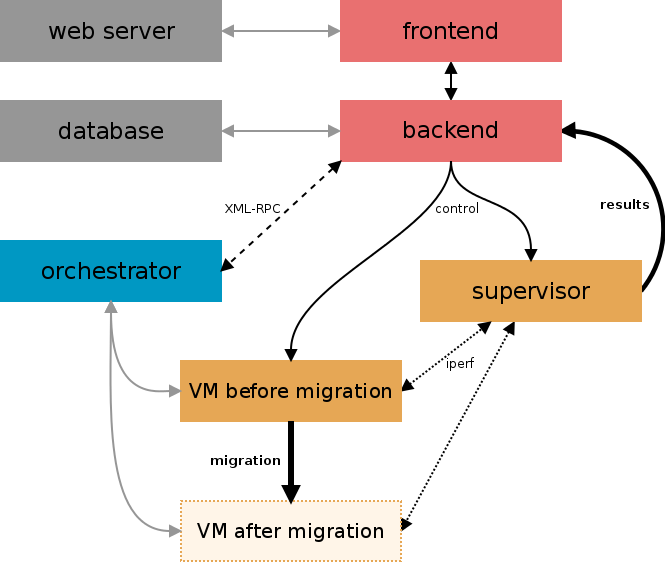
\includegraphics[width=0.7\textwidth]{themis-model.png}
	\end{center}
	\caption{Model of Themis application}
	\label{img:themis-model}
\end{figure}



% languages
Application is written in Ruby using Ruby on Rails framework. Ruby is platform independent and can run on every currently used operating system. Ruby on Rails (\Ac{RoR}) is framework providing database abstraction and strictly based on model-view-controller (\Ac{MVC}) architecture. Application is based on object model, outputs are generatied using views and controller is responsible for sending commands to models and forward results to views.

I have decided to use this framework because it provides better interaction with system services, e.g. \Ac{SSH} and \Ac{SCP}, than other web frameworks. There are public available classes for interaction with OpenNebula and OpenStack cloud \Ac{API} so it is not necessary to create \mbox{\Ac{XML}-\Ac{RPC}} parsers from scratch.
